\section{Auswertung}
\subsection{Bestimmung der g-Faktoren und Horizontalkomponente der Erdmagnetfeld}
Zu Beginn wird die lokale horizontal Komponente des Erdmagnetfeldes und die Lande-Faktoren $g_F$ der Rb-Isotope, welche in der Dampfzelle enthalten sind, ermittelt.
Dafür werden die verschiedenen Frequenzen gegen die magnetischen Feldstärken in der jeweiligen Resonanz aufgetragen. Mittels einer linearen Ausgleichsrechnung werden die $g_F$ als Steigung und die horizontal Komponente als Ordinate identifiziert.

\begin{figure}[h]
\centering
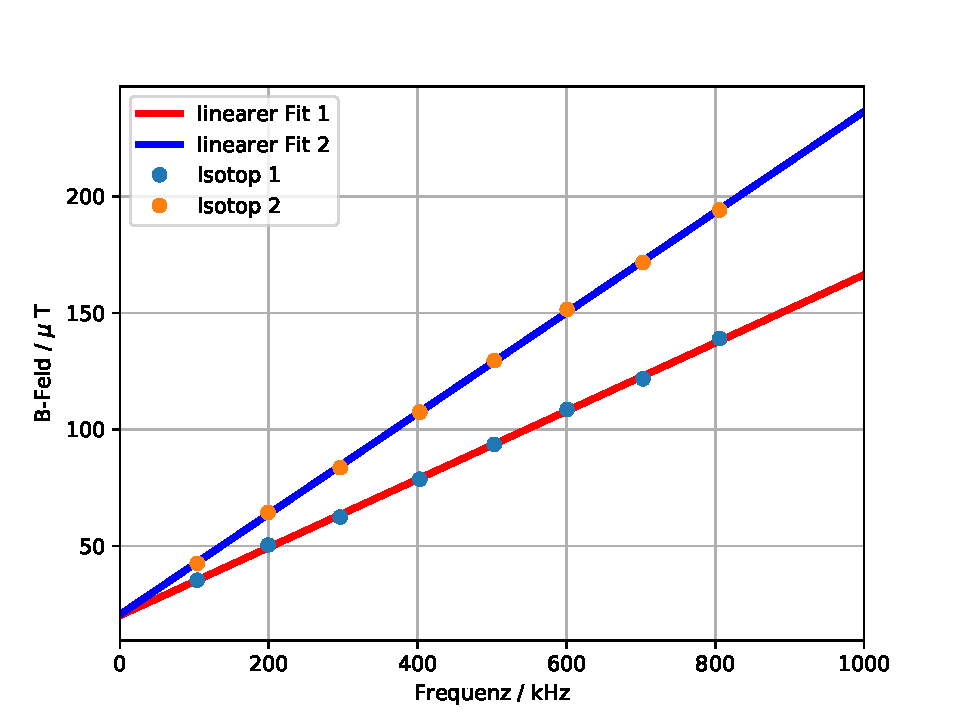
\includegraphics[scale=0.8]{./optischesPumpen/img/plotLande.pdf}
\caption{Ausgleichsrechnung zur Bestimmung der Lande Faktoren der Rb-Isotope und der lokalen horizontal Komponente des Erdmagnetfeldes}
\label{aufbau}
\end{figure}

Mit dem Ansatz
\begin{equation}
f(x) = Ax + B
\end{equation}
folgt aus der Ausgleichsrechnung folgende Werte für die Koeffizienten A und B.

\begin{table}\centering\begin{tabular}{ccc} \toprule 
\centering
\caption{Ergebnisse für die Koeffizienten A und B der Ausgleichsrechnung.}
\label{tab:isoFit}
 & A / $\mu$T/kHz  & B / $\mu$T \\ \midrule
Isotop 1 & 0.146 $\pm$ 0.001 & 20.1 $\pm$ 0.7 \\
Isotop 2 & 0.216 $\pm$ 0.001 & 20.5 $\pm$ 0.6 \\
\bottomrule
\end{tabular}
\end{table}

Durch Koeffizientenvergleich mit gleichung 0.10 folgt für die Lande Faktoren

\begin{equation} 
g_{F1} = 0.488\pm0.005\,
label{eq:resG1}
\end{equation} 


und

\begin{equation} 
g_{F2} = 0.331\pm0.002\,
label{eq:resG2}
\end{equation} 


Außerdem lässt sich aus der Ordinate die horizontalkomponente des Erdmagnetfeldes bestimmen,
welche sich zu

\begin{equation} 
B_\text{h} = 20.3\pm0.5\,\mu\text{T}
\end{equation} 


errechnet.

\subsection{Bestimmung der Kernspins}
Zur bestimmung des Kernspins muss Gleichung (?) für die zwei berechneten g-Faktoren gelöst werden. Dafür werden beide Seiten der Gleichung in Abhängigkeit
des Kernspins I aufgetragen. Der Punkt an den sich beide Kurven schneiden, zeigt den Kernspin des zu Untersuchenden Isotope an.

\begin{figure}[H]
\centering
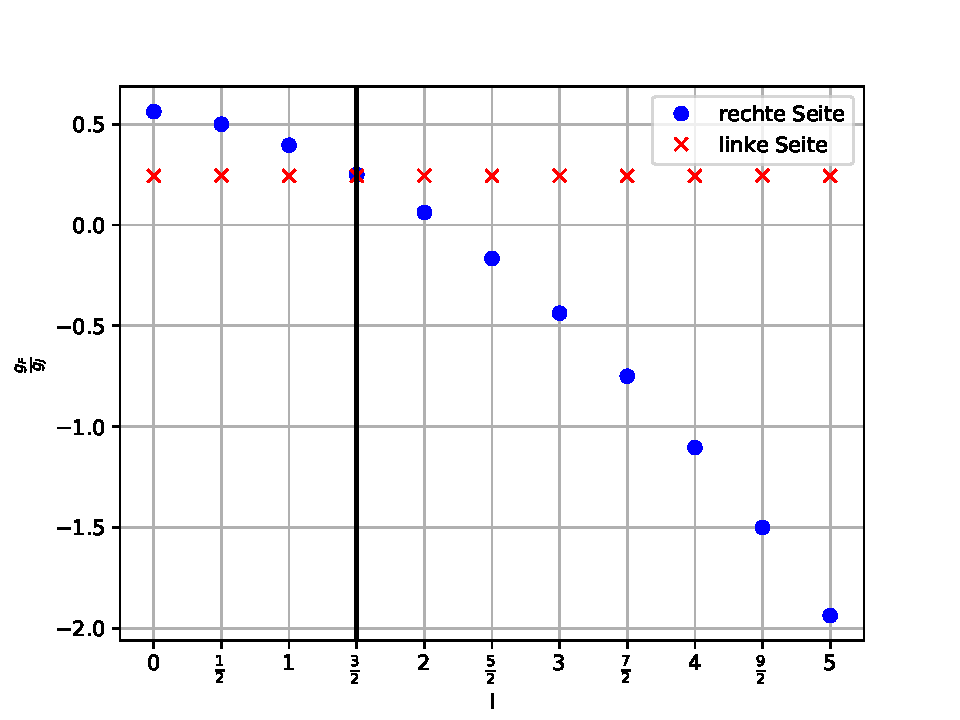
\includegraphics[scale=0.8]{./optischesPumpen/img/coreSpin1.pdf}
\caption{Ausgleichsrechnung zur Bestimmung der Lande Faktoren der Rb-Isotope und der lokalen horizontal Komponente des Erdmagnetfeldes}
\label{aufbau}
\end{figure}

\begin{figure}[H]
\centering
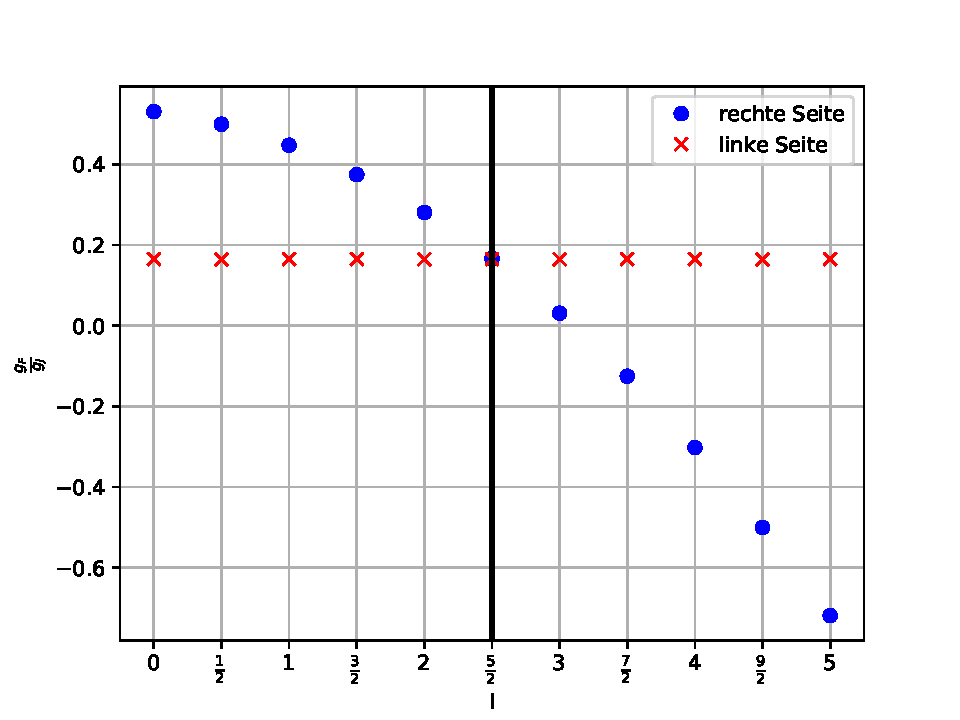
\includegraphics[scale=0.8]{./optischesPumpen/img/coreSpin2.pdf}
\caption{Ausgleichsrechnung zur Bestimmung der Lande Faktoren der Rb-Isotope und der lokalen horizontal Komponente des Erdmagnetfeldes}
\label{aufbau}
\end{figure}

Aus den errechneten g-Faktoren und Kernspins können wir Isotop 1 als Rb87 und Isotop 2 als Rb85 identifizieren.


\subsection{Bestimmung des Isotopenverhältnisses}
In Abbildung (?) ist das Signalbild dargestellt, welches die Resonanzen zu festen
Feldstärken zeigt.

\begin{figure}[H]
\centering
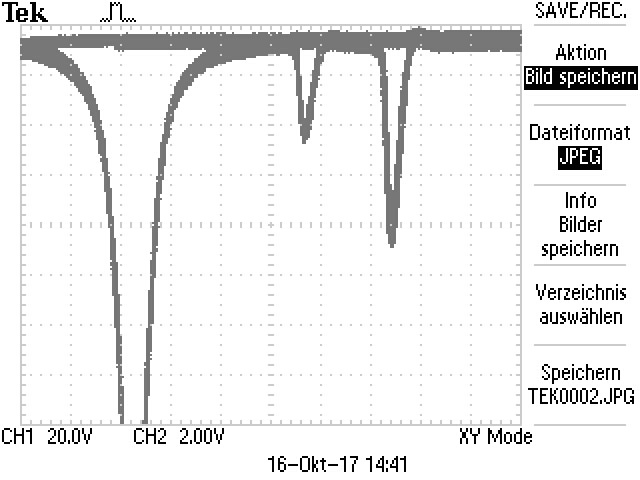
\includegraphics[scale=0.8]{./optischesPumpen/img/TEK0002.JPG}
\caption{Ausgleichsrechnung zur Bestimmung der Lande Faktoren der Rb-Isotope und der lokalen horizontal Komponente des Erdmagnetfeldes}
\label{aufbau}
\end{figure}


Aus dem Amplitudenverhältnis der Resonanzen wird das Isotopenverhältnis in der
Dampfzelle ermittelt. Dafür wird die Tiefe der Resonanzen in Pixel bestimmt.
Eine Messung der Tiefe der Resonanzen mit gimp liefert für die erste Resonanz (von links)

\begin{equation} 
h_1 = 108.0\pm1.1\,\text{px}
\end{equation} 


für die zweite Resonanz

\begin{equation} 
h_2 = 213.0\pm2.1\,\text{px}
\end{equation} 


und für das Amplitudenverhältnis

\begin{equation} 
r = 0.507\pm0.007\,
\end{equation} 


Bei der Kalkulation des Amplitudenverhältnisses wurde ein Ablesefehler von 1 Prozentpunkt
angesetzt.

\subsection{Abschätzung des quadratischen Zeemann-Effektes}
Für starke Magnetfelder verhält sich die Übergangsenergie $U_{HF}$ nicht mehr proportional zu B, um diese Abweichung zu berücksichtigen, ist es notwenig Terme höherer Ordnung zu betrachten.
Im folgenden wird die größe des quadratischen Termes für die genutzen Feldstärken abgeschätzt. Wird der quadratische Term explizit ausgewertet zeigt sich, dass der quadratische Zeeman-Effekt
in diesem Fall proportional zu $10^{-33}$ ist.
